\section{Box-counting dimenze}\label{sec:box-counting-dimenze}

Tomuto typu dimenze jsme se již v~základu věnovali v~kapitole~\ref{chapter:uvod_do_fraktalu},~specificky sekci~\ref{sec:fraktalni_dimenze},~kde jsme rozebrali způsob jejího výpočtu a~ukázali jsme si jej několika příkladech. V~této části si blíže rozebereme některé další vlastnosti týkající se právě \emph{box-counting dimenze}\index{box-counting dimenze}\index{dimenze!box-counting}\footnote{V kapitole~\ref{chapter:uvod_do_fraktalu} jsme pro jednoduchost používali obecnější termín \emph{fraktální dimenze}. Ten však zahrnuje daleko širší škálu možných definic,~než jen tu,~kterou jsme si představili. Avšak dále v~tomto textu budeme používat výhradně její skutečný název,~tj. box-counting dimenze.} a~pokusíme se ji lépe zasadit do kontextu teorie míry,~které jsme se samostatně až do této chvíle věnovali.

\subsection{Definice a~výpočet}\label{subsec:definice-a-vypocet-bc-dimenze}

Jako první se podíváme na myšlenku box-counting trochu blíže a~maličko si ji zobecníme. Původně jsme nahlíželi na dimenzi jako na exponent,~s nímž roste "velikost" zkoumaného útvaru. Tato myšlenka se ukázala jako rozumná,~neboť pro "klasické" geometrické útvary vycházela tato dimenze vždy celočíselně,~nicméně už tomu tak nebylo v~případě fraktálních útvarů. Podstata byla taková,~že jsme útvar $F$ rozdělili na určitý počet stejně "velkých částí",~označme je $F_1,F_2,\ldots,F_m$ v~nějakém měřítku $\varepsilon>0$. Zkusme nyní požadavek na striktně stejnou velikost (formálně vzato míru) trochu rozvolnit. Bude nám stačit,~když pro každé $i$ je
\[\diam{F_i}\leqslant\delta,\;\text{kde}\;\delta>0.\]
Zároveň nebudeme požadovat,~aby množiny $F_1,F_2,\ldots,F_m$ byly všechny po dvou téměř disjunktními\footnote{Množiny $M,N$ jsou \emph{téměř disjunktní},~pokud $\interior{M}\cap\interior{N}=\emptyset$,~tedy může nastat,~že se na hranici mohou "dotýkat",~tzn. $\boundary{M}\cap\boundary{N}\neq\emptyset$.} podmnožinami $F$,~ale stačí,~když budou tvořit pokrytí $F$.

Mějme tedy nějakou neprázdnou omezenou množinu $F\subset\R^n$,~kde pro každé $\delta>0$ budeme hledat \emph{nejmenší počet} množin pokrývajících $F$. Toto číslo si označíme $N_\delta(F)$. Dimenze množiny $F$ by tedy měla odrážet "rychlost" růstu $N_\delta(F)$ pro $\delta\to 0_+$. Je-li splněna aproximace
\begin{equation}\label{eq:odhad-n-delta}
    N_\delta(F)\approx c\delta^{-s}
\end{equation}
pro $c>0$,~pak řekneme,~že množina $F$ má box-counting dimenzi $s$. (Převzato z~\citep[str. 27]{Falconer2014}.)
\begin{remark}
    V~dalším textu budeme místo $\delta\to 0_+$ psát pro jednoduchost pouze $\delta\to 0$,~byť by se slušilo používat první variantu. Čtenáři je však nejspíše jasné,~že uvažovat záporný průměr množiny nemá smysl.
\end{remark}
Logaritmováním a~úpravou výrazu \eqref{eq:odhad-n-delta} dostaneme:
\begin{align}\label{eq:odvozeni-box-counting-dimenze}
    \ln{N_\delta(F)}&\approx\ln{c}+\ln{\delta^{-s}}\\
    \ln{N_\delta(F)}&\approx\ln{c}-s\ln{\delta}\\
    s&\approx\dfrac{\ln{N_\delta(F)}}{-\ln{\delta}}+\dfrac{\ln{c}}{\ln{\delta}}.
\end{align}
Když porovnáme výsledek v~\eqref{eq:odvozeni-box-counting-dimenze} s~rovností \eqref{eq:fraktalni-dimenze} z~minulé kapitoly,~můžeme si všimnout,~že zde navíc figuruje člen $\ln{c}/\ln{\delta}$. Když však uvážíme limitu daného výrazu pro $\delta\to 0$,~dostaneme původní vzorec,~který jsme již viděli,~tj.
\[\lim_{\delta\to 0}\left(\dfrac{\ln{N_\delta(F)}}{-\ln{\delta}}+\dfrac{\ln{c}}{\ln{\delta}}\right)=\lim_{\delta\to 0}\dfrac{\ln{N_\delta(F)}}{-\ln{\delta}}+\lim_{\delta\to 0}\dfrac{\ln{c}}{\ln{\delta}}=\lim_{\delta\to 0}\dfrac{\ln{N_\delta(F)}}{-\ln{\delta}}.\]
% \begin{definition}[$\delta$-pokrytí]\label{def:delta-pokryti}
%     Nechť $(X,\varrho)$ je metrický prostor,~$F\subseteq X$ a~$\delta>0$. Jestliže $\mathcal{F}=\set{F_1,F_2,\ldots}\subseteq\powset{X}$ je pokrytí $F$ a~zároveň $\diam{F_j}\leqslant\delta$ pro každé $j$,~pak $\mathcal{F}$ nazýváme $\delta$-pokrytí\index{$\delta$-pokrytí} množiny $F$.
% \end{definition}
Předchozí úvahu můžeme shrnout do následující definice.
\begin{definition}[Box-counting dimenze]\label{def:box-counting-dimenze}
    Nechť $F\subset \R^n$ je neprázdná omezená množina. Pak definujeme následující:
    \begin{enumerate}[label=(\alph*)]
        \item \emph{Nejmenší počet množin v~$\delta$-pokrytí množiny $F$} značíme $N_\delta(F)$,~tj.
        \[N_\delta(F)=\min\set{m\in\N\;\middle|\;F\subseteq\bigcup_{i=1}^m F_i\;,\;\diam{F_j}\leqslant\delta\;\text{pro}\;1\leqslant j\leqslant m}.\]
        \item \emph{Horní box-counting dimenze}\index{box-counting dimenze!horní}\index{horní box-counting dimenze} množiny $F$ je
        \[\upperdimB{F}=\limsup_{\delta\to 0}\dfrac{\ln{N_\delta(F)}}{-\ln{\delta}}.\]
        \item \emph{Dolní box-counting dimenze}\index{box-counting dimenze!dolní}\index{dolní box-counting dimenze} množiny $F$ je
        \[\lowerdimB{F}=\liminf_{\delta\to 0}\dfrac{\ln{N_\delta(F)}}{-\ln{\delta}}.\]
    \end{enumerate}
    V~případě,~že $\lowerdimB{F}=\upperdimB{F}$,~pak společnou hodnotu nazýváme \emph{box-counting dimenzí}\index{dimenze!box-counting}\index{box-counting dimenze} množiny $F$,~značíme $\dimB{F}$,~přičemž platí
    \[\dimB{F}=\lim_{\delta\to 0}\dfrac{\ln{N_\delta(F)}}{-\ln{\delta}}.\]
\end{definition}
\begin{remark}
    Zde je důležité zmínit,~že v~dalším textu budeme uvažovat $\delta$ dostatečně malé,~konkrétně $0<\delta<1$,~tzn.~hodnota $-\ln{\delta}$ je~vždy kladná. Dále budeme pracovat (podle definice~\ref{def:box-counting-dimenze}) pouze s~neprázdnými omezenými množinami,~abychom se vyhnuli problémům s~případy,~kdy "$N_\delta(F)=\infty$" nebo $N_\delta(F)=0$. Každá omezená množina v $\R^n$ je totiž obsažena v~nějaké kompaktní množině,~tzn. vždy nám postačí konečně mnoho množin o~průměru nejvýše $\delta$ k~jejímu pokrytí.
\end{remark}
pro úplnost ještě zmíníme,~že box-counting dimenzi lze taktéž definovat více způsoby. V~tuto uvažujeme obecně $\delta$-pokrytí dané množiny $F$,~tj. pokrytí \emph{obecnými} množinami o~průměru maximálně $\delta>0$. Lze se však zaměřit i~na konkrétní útvary,~jak ukazuje následující věta.
\begin{theorem}[Ekvivalentní definice box-counting dimenze]\label{thm:ekvivalentni-def-box-counting-dimenze}
    Nechť $F\subset \R^n$ je neprázdná omezená množina. Pak
    \begin{align*}
        \lowerdimB{F}&=\liminf_{\delta\to 0}\dfrac{\ln{M_\delta(F)}}{-\ln{\delta}},\\
        \upperdimB{F}&=\limsup_{\delta\to 0}\dfrac{\ln{M_\delta(F)}}{-\ln{\delta}},\\
        \dimB{F}&=\lim_{\delta\to 0}\dfrac{\ln{M_\delta(F)}}{-\ln{\delta}},
    \end{align*}
    kde $M_\delta(F)$ je definováno jedním z~následujících vzorců:
    \begin{enumerate}[label=(\roman*)]
        \item\label{thm:pokryti-delta-uz-koulemi} $\displaystyle M_\delta(F)=\inf\set{m\;\middle|\;F\subseteq\bigcup\limits_{i=1}^m K_\delta(x_i)\;,\;x_j\in\R^n\;\text{pro}\;1\leqslant j\leqslant m}$;
        \item\label{thm:pokryti-delta-kvadry} $\displaystyle M_\delta(F)=\inf\set{m\;\middle|\;F\subseteq\bigcup\limits_{i=1}^m I_i\;,\;I_j=\prod_{k=1}^{n}\langle a_k,a_k+\delta\rangle\;\text{pro}\;1\leqslant j\leqslant m}$;
        \item\label{thm:pokryti-delta-sit} $\displaystyle M_\delta(F)=\left|\set{I\;\middle|\;I\cap F\neq\emptyset\;,\;I\in\mathcal{Q}_\delta}\right|$,~kde $\delta>0$;
        \item\label{thm:pokryti-delta-dis-ot-koulemi} $\displaystyle M_\delta(F)=\sup\set{m\;\middle|\;B_\delta(x_i)\cap B_\delta(x_j)=\emptyset\;;\;x_i,x_j\in\R^n\;\text{pro}\;1\leqslant i,j\leqslant m}$.
    \end{enumerate}
\end{theorem}

Nyní si pojďme větu~\ref{thm:ekvivalentni-def-box-counting-dimenze} trochu rozebrat.
\begin{itemize}
    \item Body~\ref{thm:pokryti-delta-uz-koulemi} a~\ref{thm:pokryti-delta-dis-ot-koulemi} říkají,~že $M_\delta(F)$ je rovno \emph{nejmenšímu počtu uzavřených koulí o~poloměru $\delta$,~které pokrývají $F$},~resp. \emph{nejvyšší počet disjunktních otevřených koulí o~poloměru $\delta$,~které mají střed v~$F$}.
    \item Podobně body~\ref{thm:pokryti-delta-kvadry} a~\ref{thm:pokryti-delta-sit} tvrdí,~že $M_\delta(F)$ lze definovat jako pokrytí kvádry o~stranách délky $\delta$,~resp. počet všech kvádrů z~$\delta$-mříže,~které mají s~$F$ neprázdný průnik.
    \item Výše zmíněné definice $M_\delta(F)$ si obecně nejsou ekvivalentní a~pevně zvolenou množinu $F$ a $\delta$ mohou dávat různé hodnoty. Hodnoty dimenzí však vyjdou (nezávisle na definici $M_\delta(F)$) vždy stejně.
\end{itemize}
Pro představu viz obrázek~\ref{fig:ilustrace-definic-bc-dimenze}. Důkaz věty je delší a~opět jej vynecháme,~nicméně lze jej nalézt v~knize \citep[str. 30]{Falconer2014}.
\begin{figure}
    \centering
    \begin{subfigure}{0.4\textwidth}
        \centering
        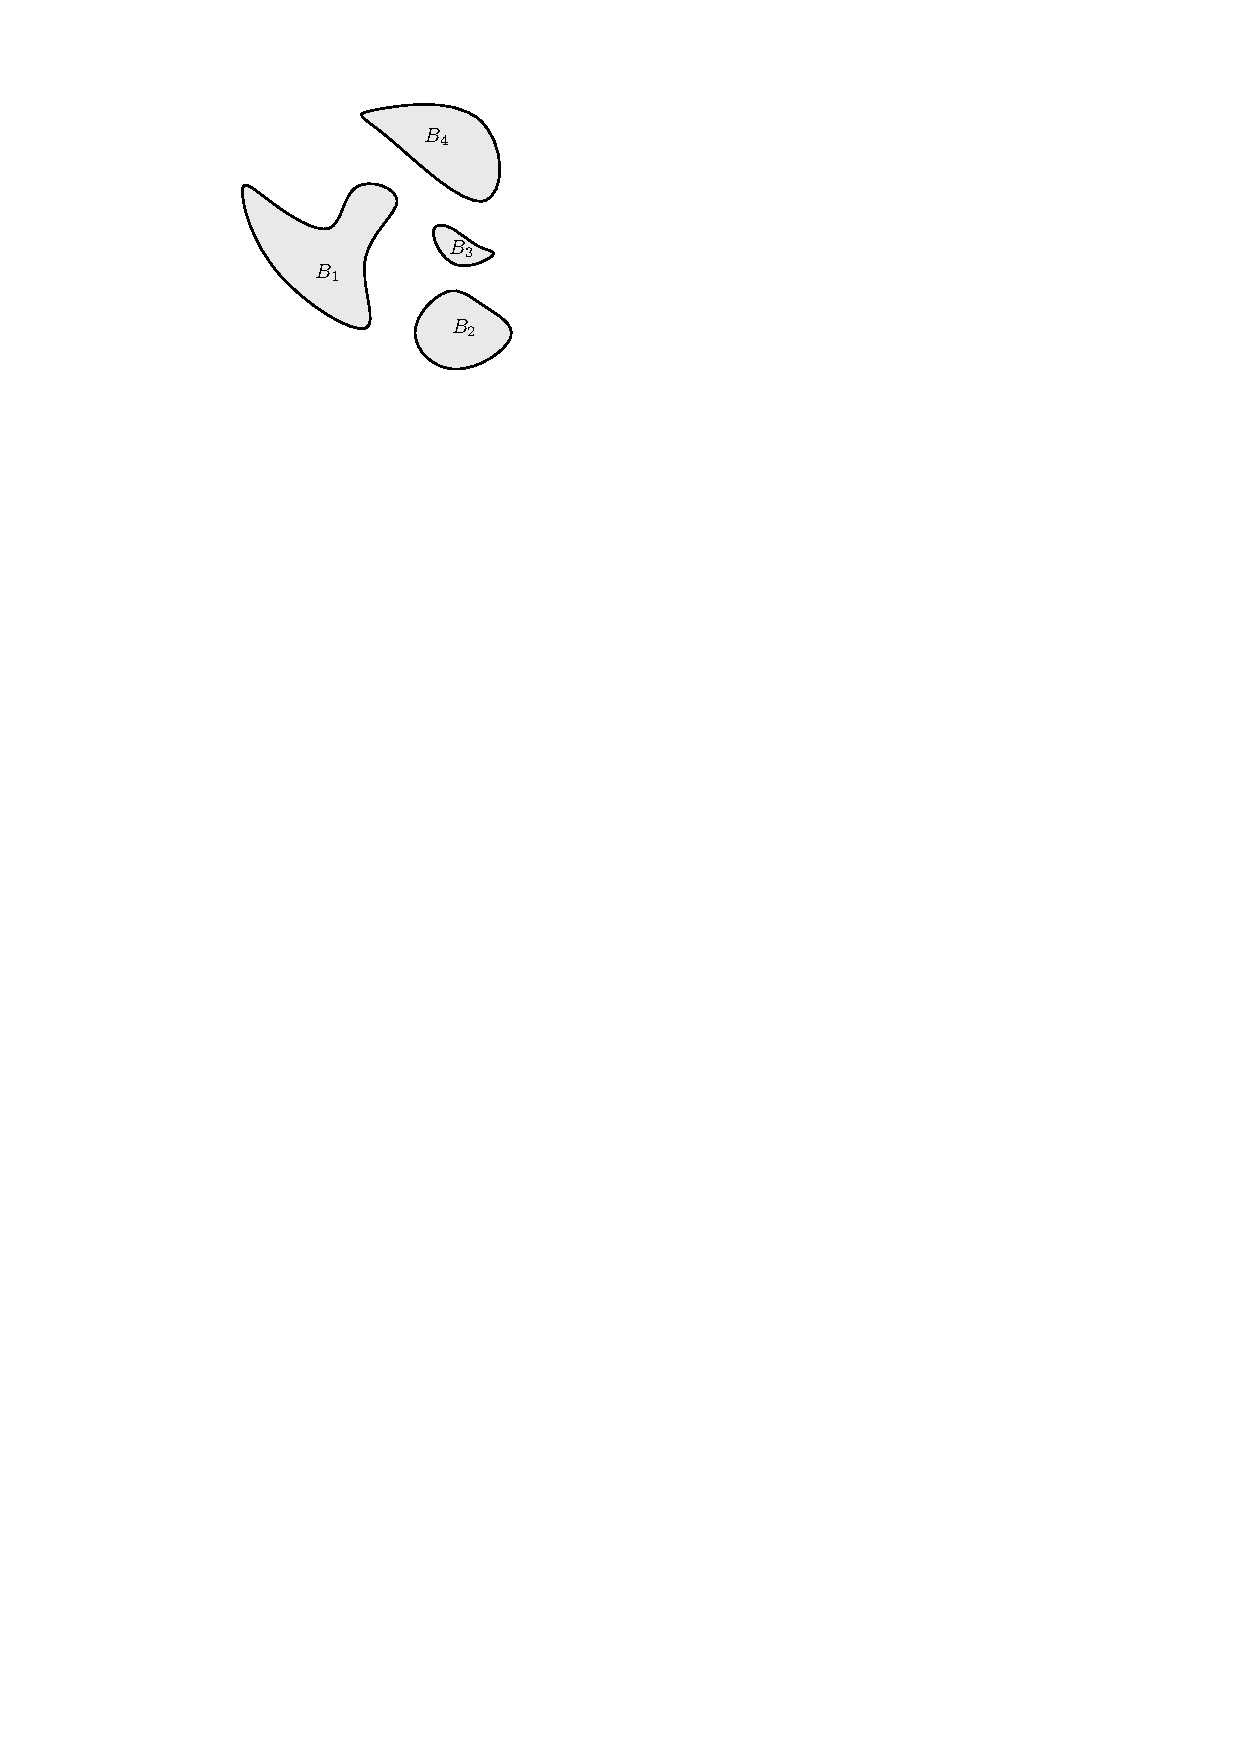
\includegraphics{ch02-bc-dimenze.pdf}
        \caption{Množina $B=\bigcup_{i=1}^4 B_i$}
        \label{subfig:bc-dimenze-pokryvana-mnozina}
    \end{subfigure}
    \qquad
    \begin{subfigure}{0.4\textwidth}
        \centering
        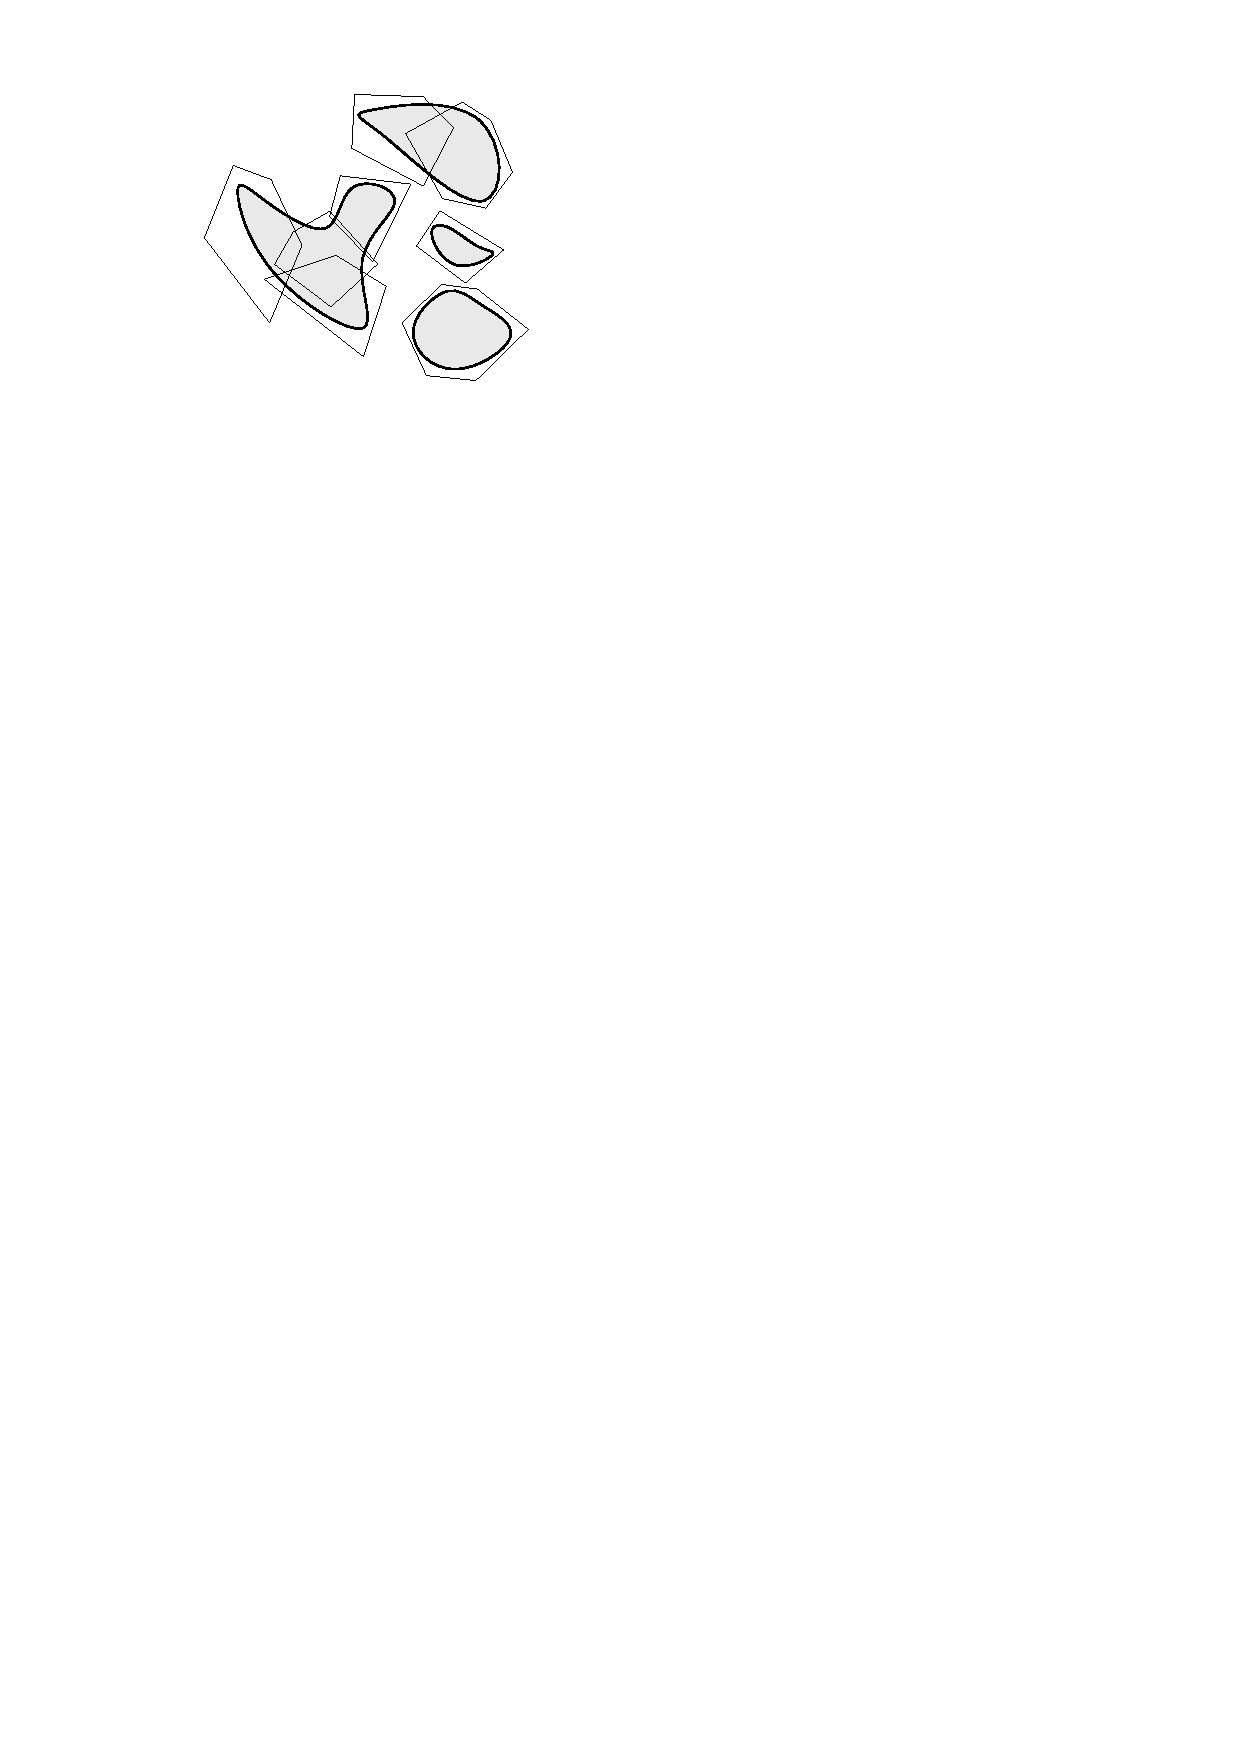
\includegraphics{ch02-bc-dimenze-delta-pokryti.pdf}
        \caption{$\delta$-pokrytí množiny $B$ (viz definice~\ref{def:box-counting-dimenze})}
        \label{subfig:bc-dimenze-delta-pokryti}
    \end{subfigure}
    \qquad
    \begin{subfigure}{0.4\textwidth}
        \centering
        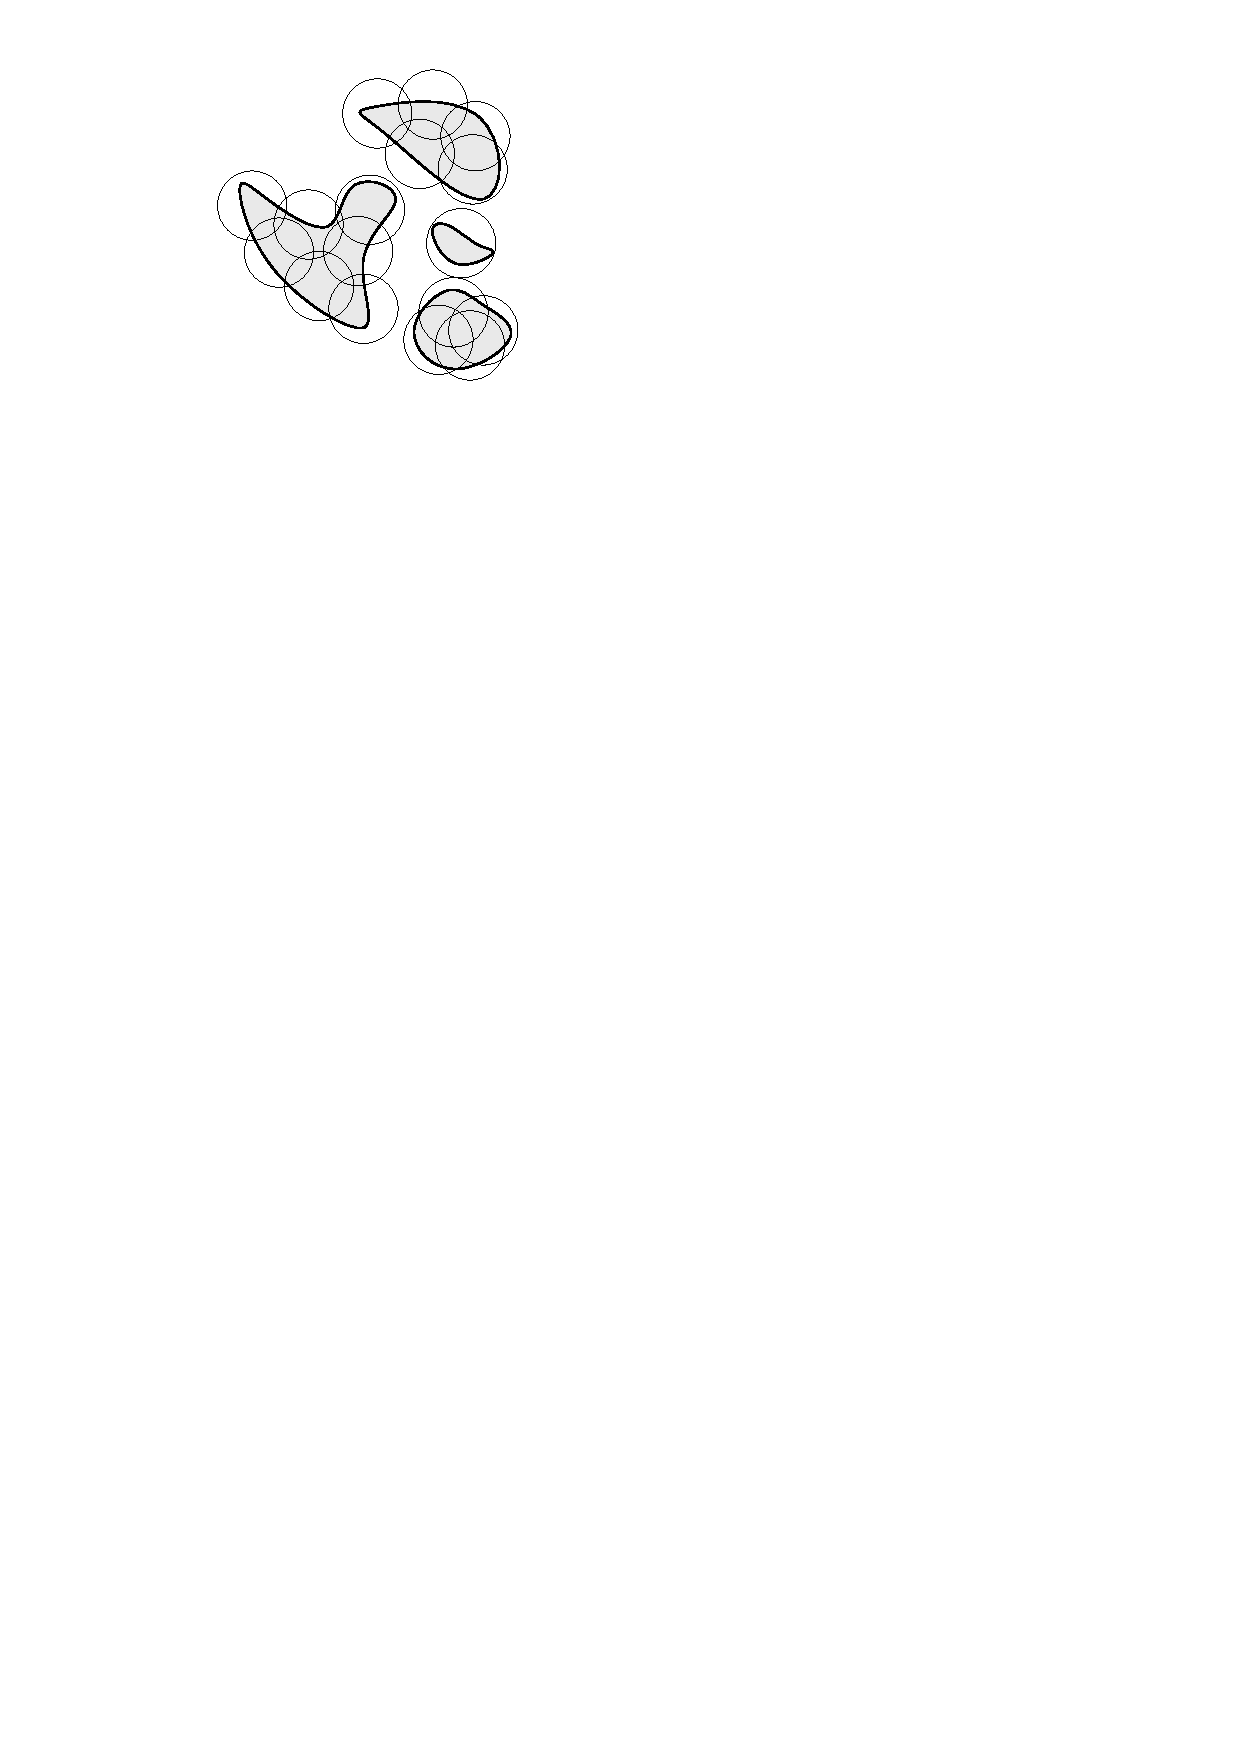
\includegraphics{ch02-bc-dimenze-pokryti-uz-koule.pdf}
        \caption{Pokrytí uzavřenými koulemi (viz bod~\ref{thm:pokryti-delta-uz-koulemi})}
        \label{subfig:bc-dimenze-uz-koule}
    \end{subfigure}
    \qquad
    \begin{subfigure}{0.4\textwidth}
        \centering
        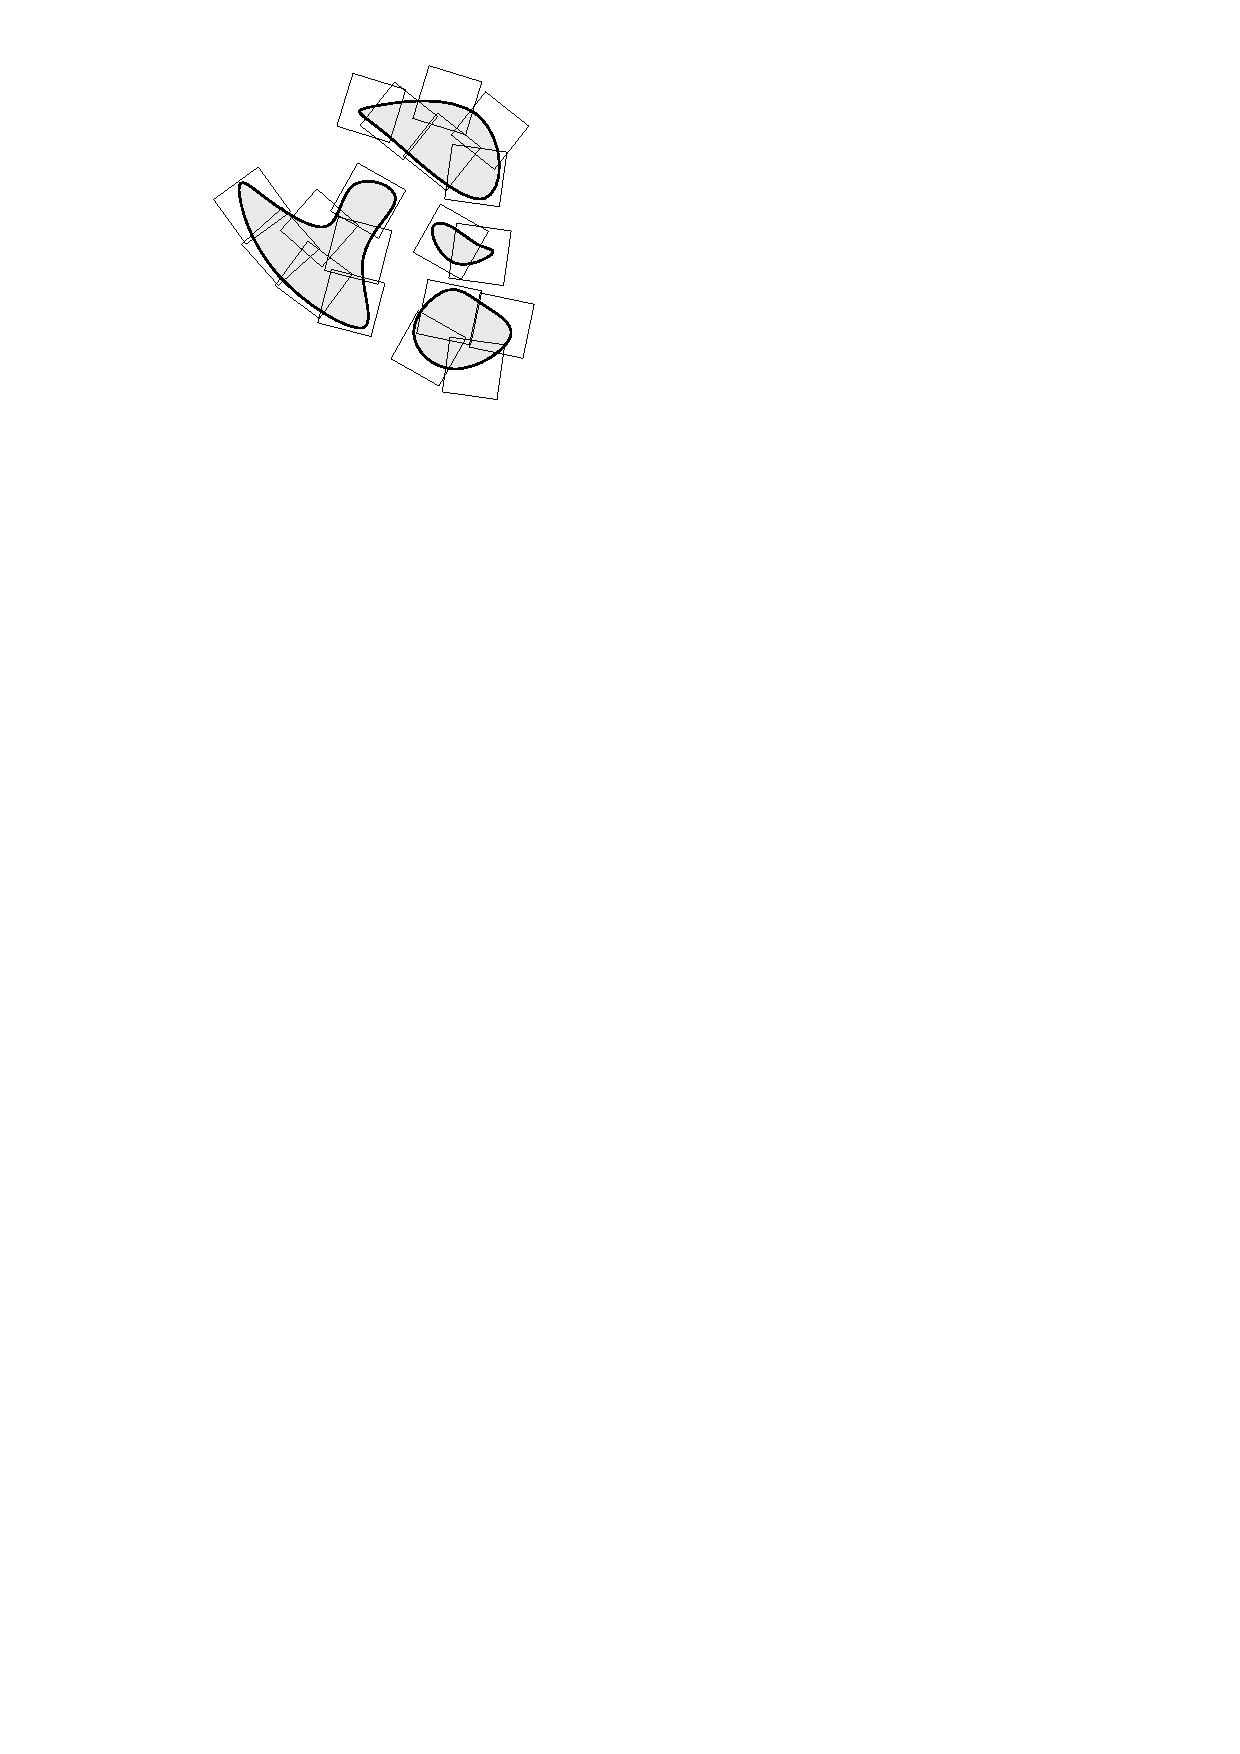
\includegraphics{ch02-bc-dimenze-pokryti-kvadry.pdf}
        \caption{Pokrytí pomocí kvádrů (viz bod~\ref{thm:pokryti-delta-kvadry})}
        \label{subfig:bc-dimenze-kvadry}
    \end{subfigure}
    \qquad
    \begin{subfigure}{0.4\textwidth}
        \centering
        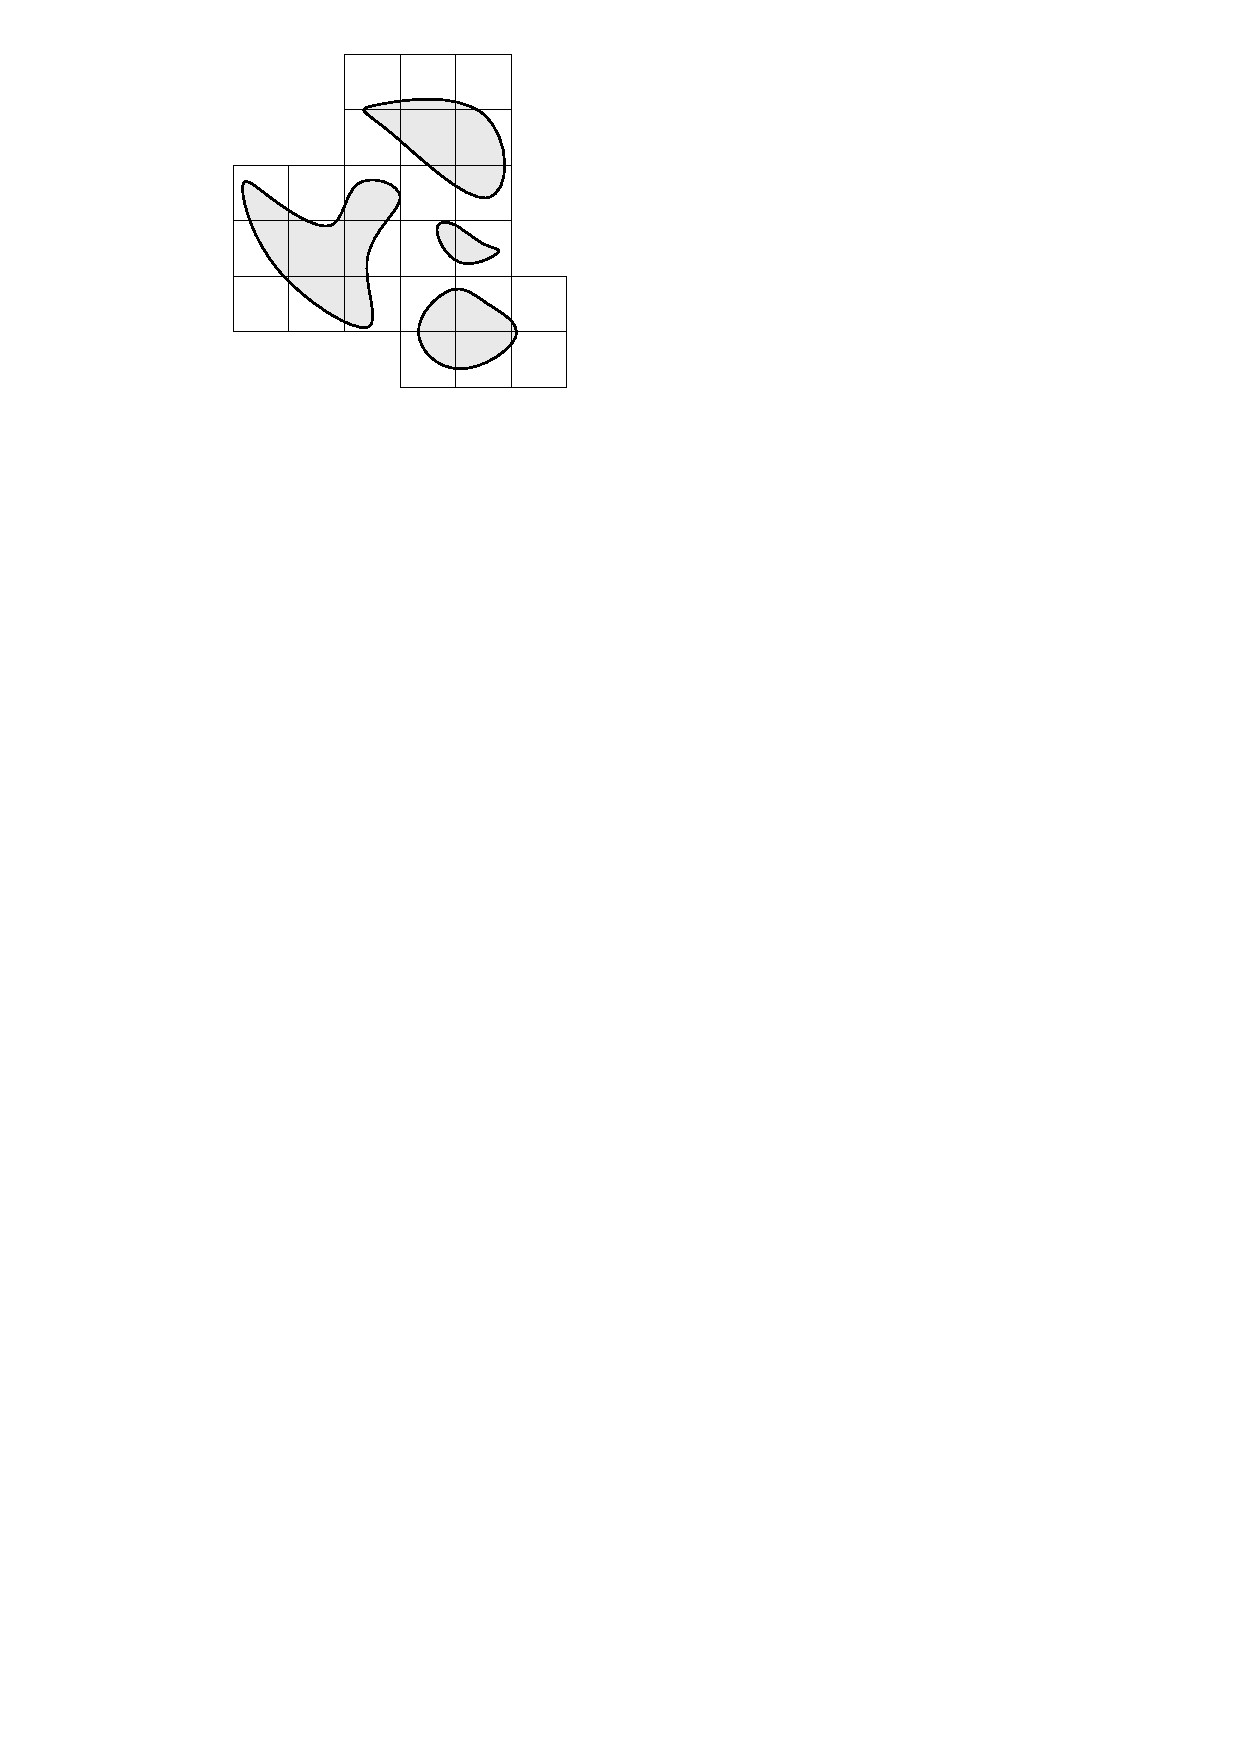
\includegraphics{ch02-bc-dimenze-pokryti-delta-sit.pdf}
        \caption{$\delta$-mříž (viz bod~\ref{thm:pokryti-delta-sit})}
        \label{subfig:bc-dimenze-delta-sit}
    \end{subfigure}
    \qquad
    \begin{subfigure}{0.4\textwidth}
        \centering
        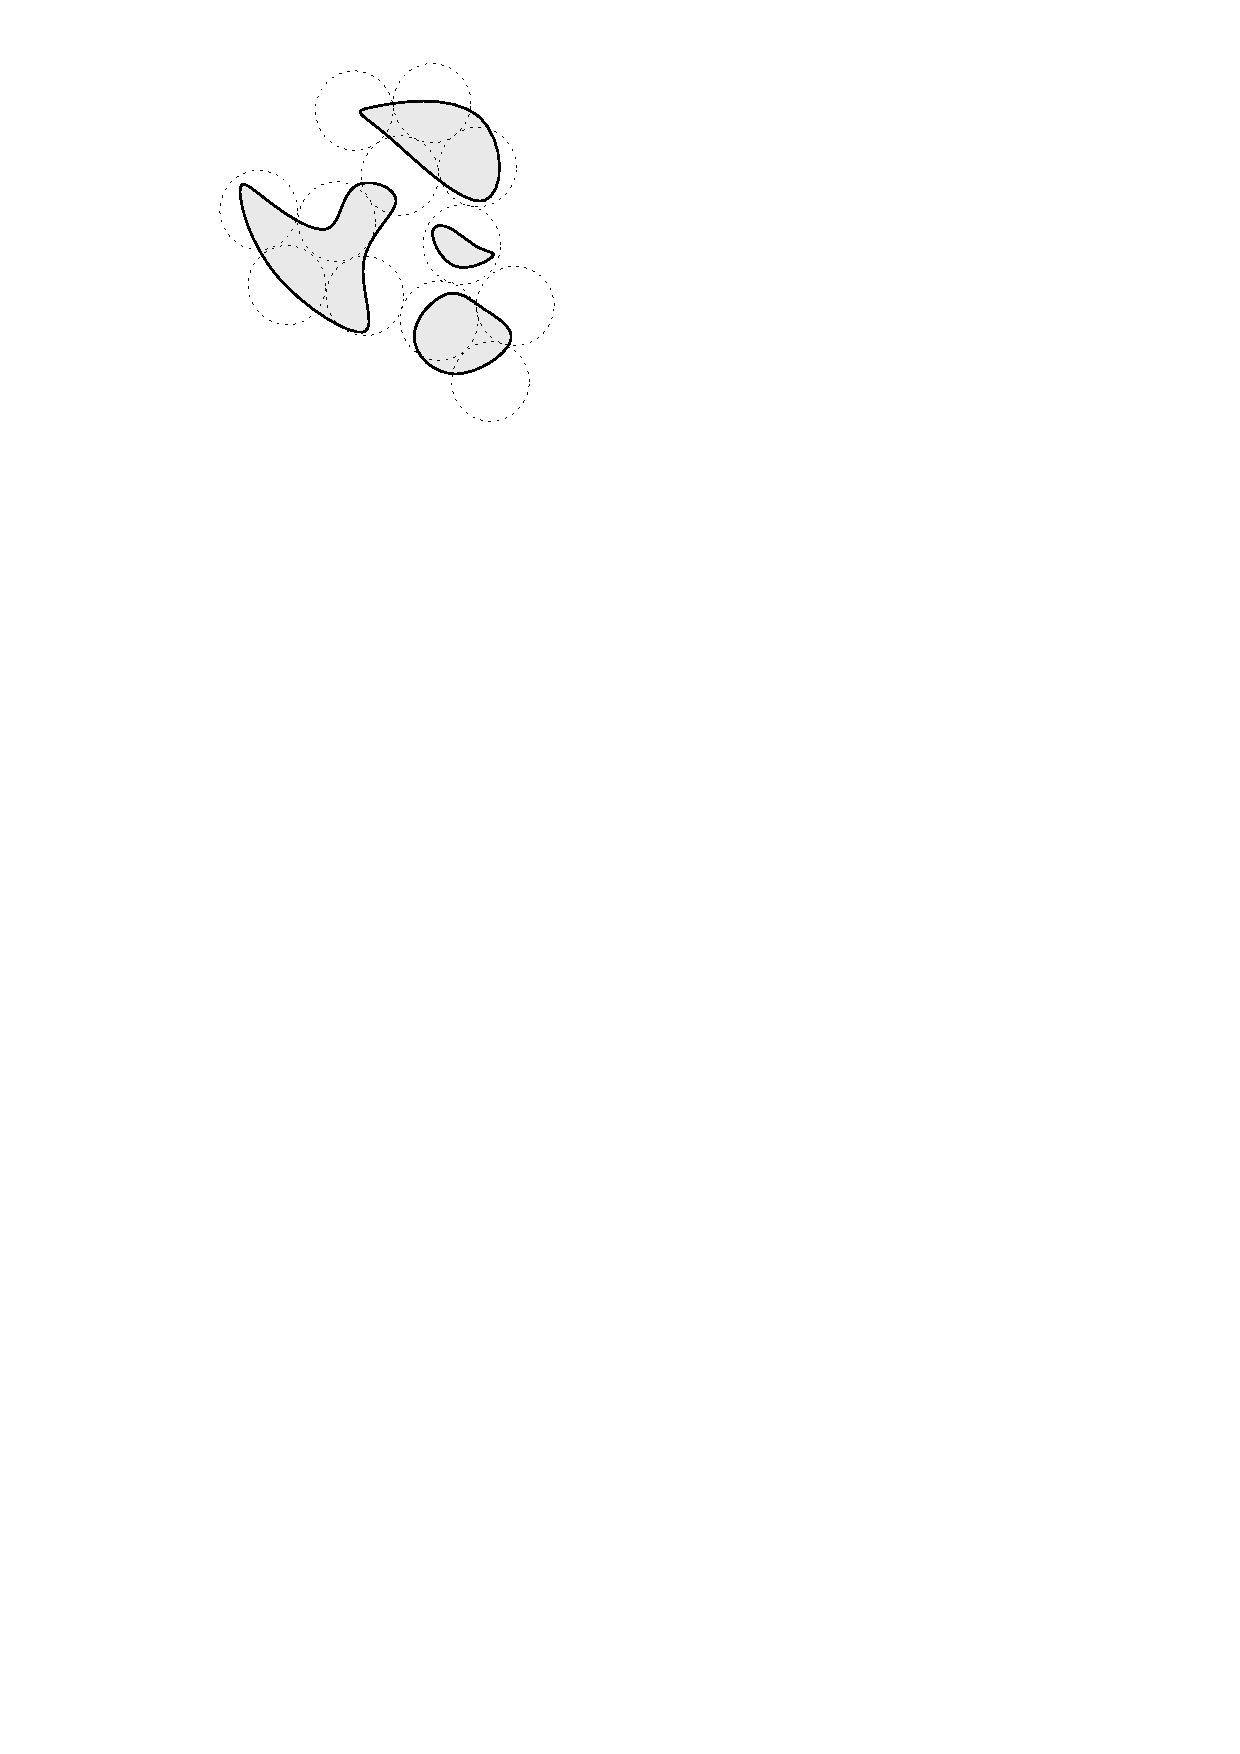
\includegraphics{ch02-bc-dimenze-pokryti-ot-koule.pdf}
        \caption{Pokrytí otevřenými po dvou disjunktními koulemi (viz bod~\ref{thm:pokryti-delta-dis-ot-koulemi})}
        \label{subfig:bc-dimenze-ot-koule}
    \end{subfigure}
    \caption[Ilustrace věty~\ref{thm:ekvivalentni-def-box-counting-dimenze}]{Ilustrace věty~\ref{thm:ekvivalentni-def-box-counting-dimenze} (Inspirováno \citep[str. 29]{Falconer2014})}
    \label{fig:ilustrace-definic-bc-dimenze}
\end{figure}

Zároveň body~\ref{thm:pokryti-delta-kvadry} a~\ref{thm:pokryti-delta-sit} nám dávají dobré opodstatnění názvu tohoto typu dimenze,~neboť v~podstatě zkoumáme pokrývání daného obrazce "kostkami". Při aproximacích box-counting dimenze obrazce $F\subset\R^2$ tak lze pracovat s~mřížkou čtverců o~libovolné straně $\delta>0$,~kdy $M_\delta(F)$ stanovíme jako počet čtverců,~které se překrývají se zkoumaným obrazcem $F$. Když se tedy zpět vrátíme k~otázce rozebírané v~úvodu tohoto textu týkající se délky pobřeží (viz kapitola~\ref{chapter:uvod_do_fraktalu}),~lze jeho "fráktálnost" do jisté míry vyjádřit právě popsaným způsobem (viz obrázek~\ref{fig:aproximace-delky-pobrezi-vb}).
\begin{figure}
    \centering
    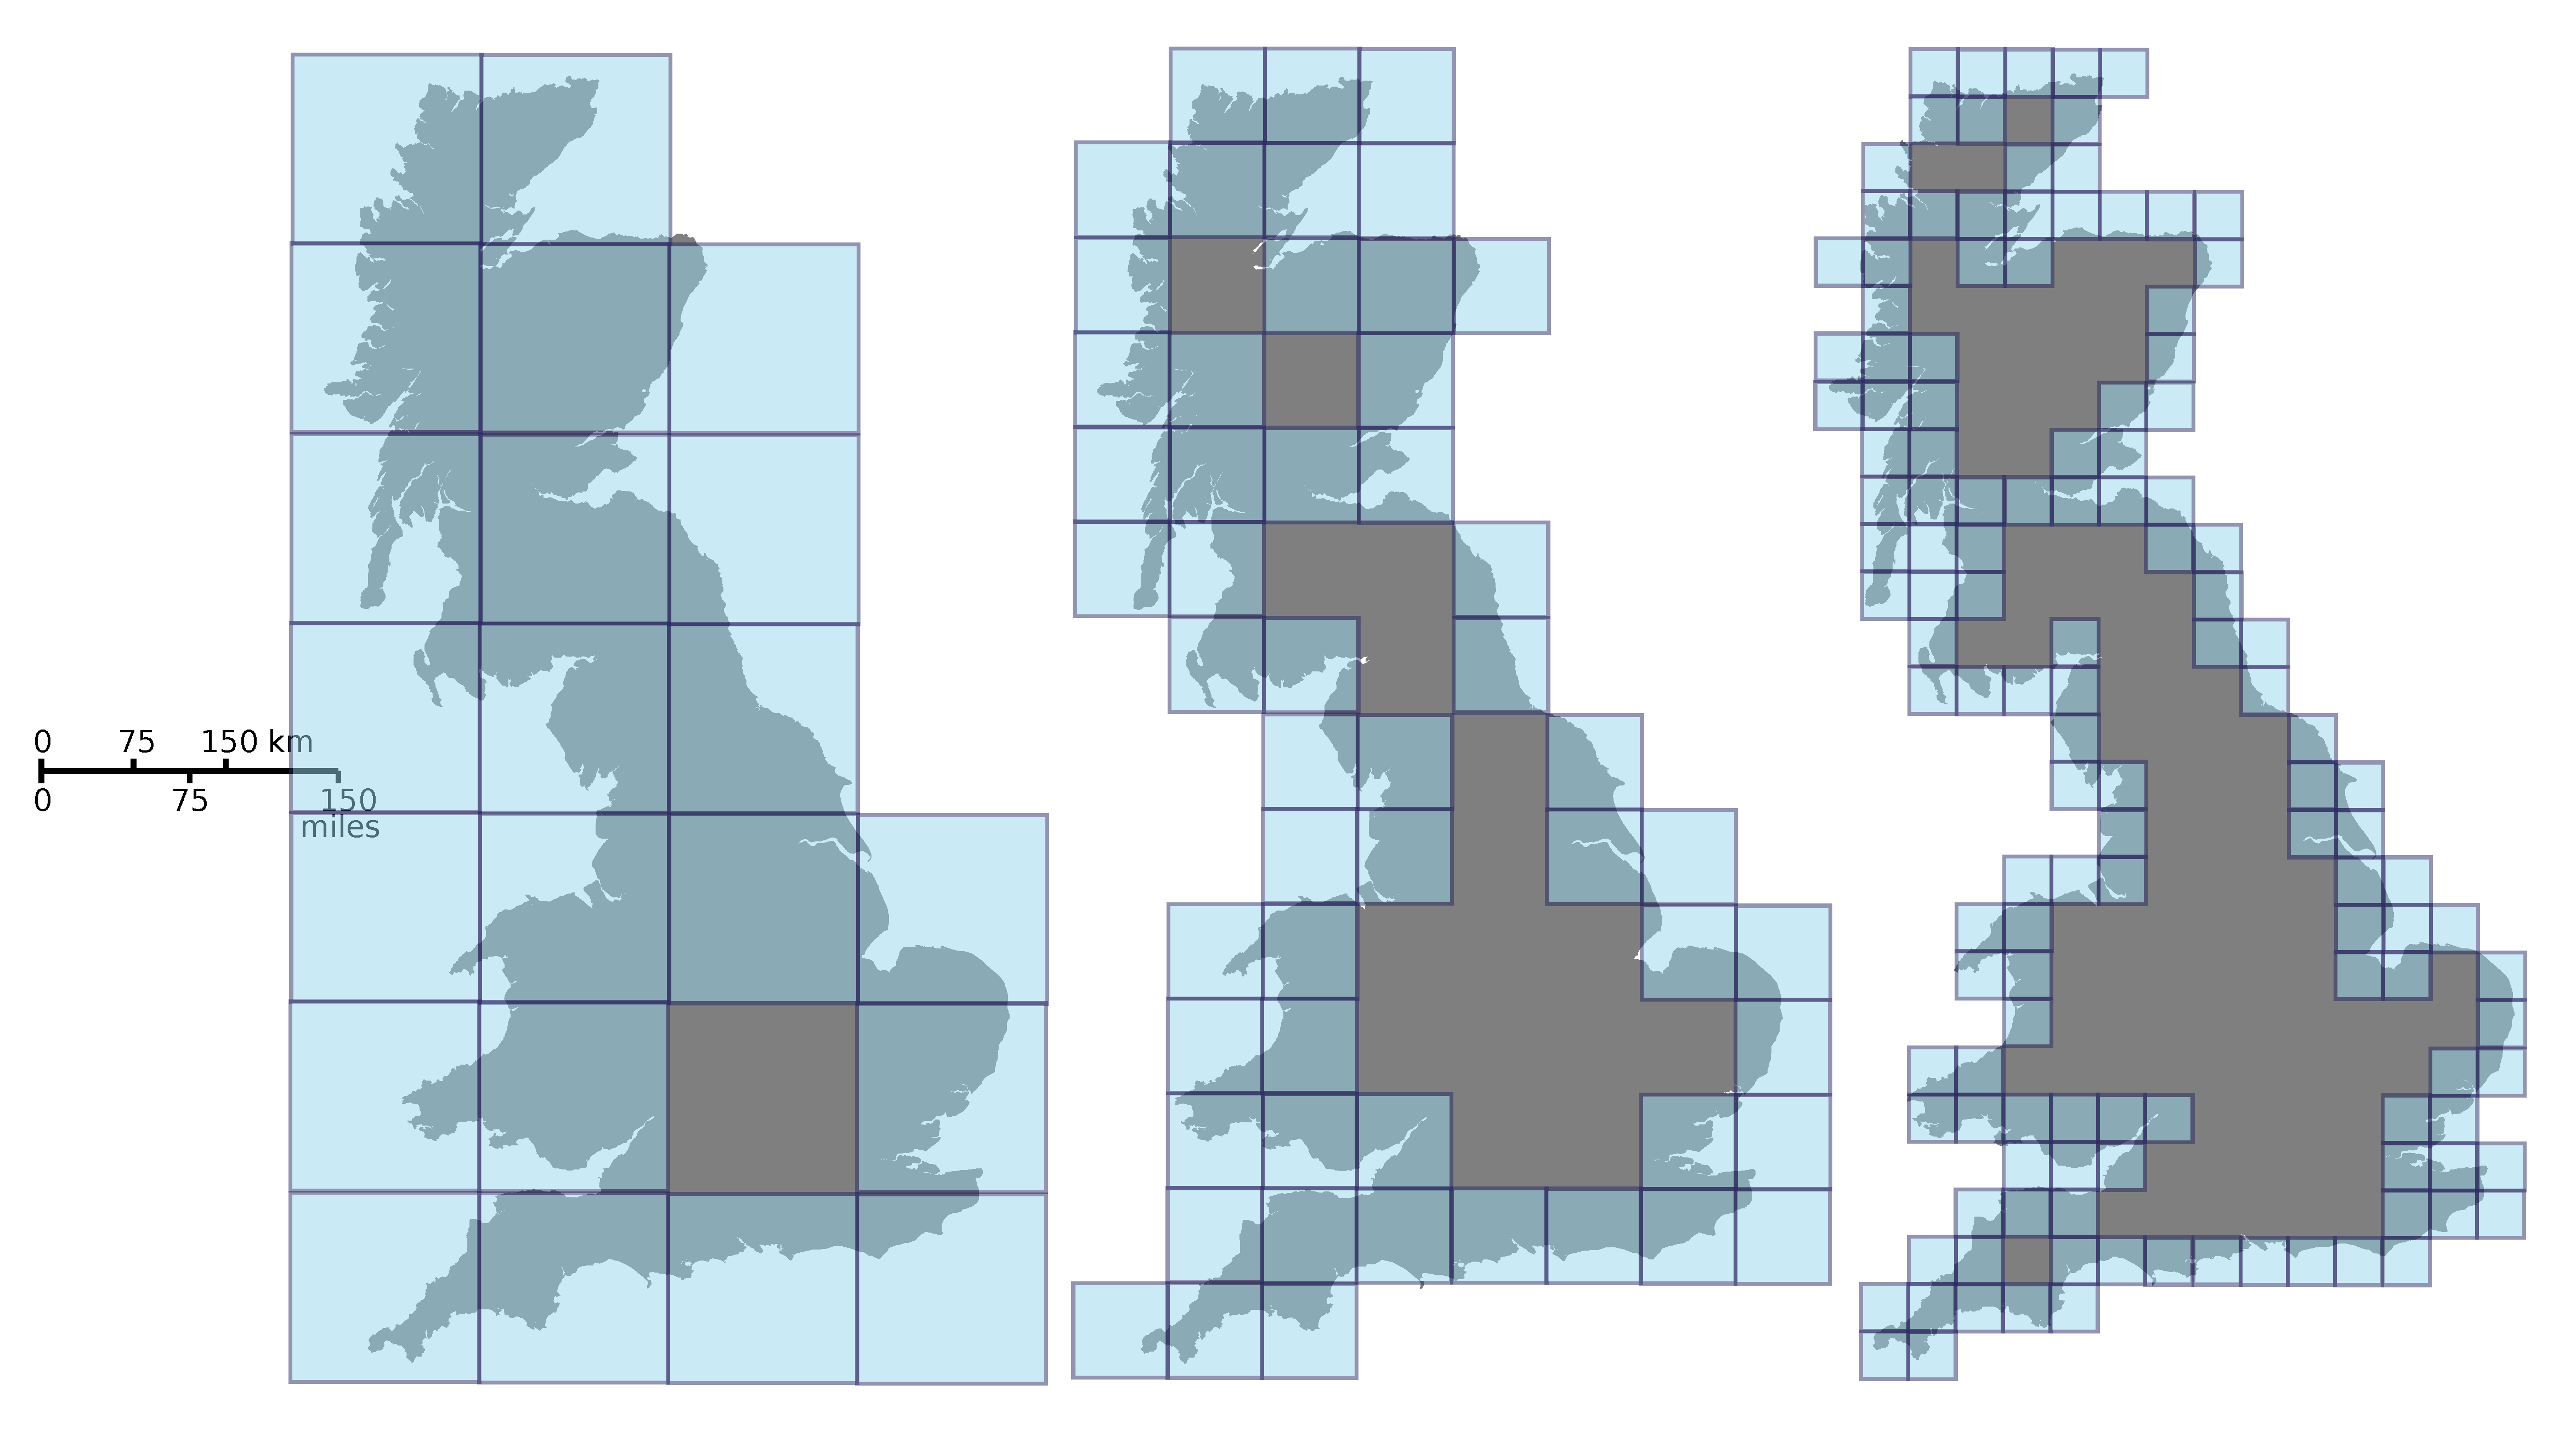
\includegraphics[width=\textwidth]{Great_Britain_Box.pdf}
    \caption[Aproximace box-counting dimenze pobřeží Velké Británie]{Aproximace box-counting dimenze pobřeží Velké Británie (Převzato z~Wikipedia Commons)\footnotemark}
    \label{fig:aproximace-delky-pobrezi-vb}
\end{figure}
Nyní se opět vrátíme k~fraktálům\footnotetext{Viz též \url{https://en.wikipedia.org/wiki/Minkowski\%E2\%80\%93Bouligand\_dimension}.} a~výpočtům jejich dimenze,~čemuž jsme se věnovali již v~podsekci~\ref{subsec:dimenze-fraktalu}. Tentokrát však budeme postupovat přímo podle definice box-counting dimenze~\ref{def:box-counting-dimenze},~tedy budeme zvlášť zkoumat horní a~dolní box-counting dimenzi.
\begin{example}[Cantorovo diskontinuum]\label{ex:cantorovo-diskontinuum}
    Formálně můžeme popsat Cantorovo diskontinuum $C$ jako průnik množin $C_k$ pro $k=0,1,2,\ldots$,~přičemž
    \[C_k=\bigcup _{j=0}^{3^{k-1}-1}\left(\left\langle{\frac {3j+0}{3^{k}}},{\frac {3j+1}{3^{k}}}\right\rangle\cup \left\langle{\frac {3j+2}{3^{k}}},{\frac {3j+3}{3^{k}}}\right\rangle\right).\]
    Platí,~že $C=\bigcap_{k=0}^\infty C_k$, přičemž $k$-tou iterací budeme rozumnět množinu $C_k=\bigcap_{i=0}^k C_i$. Již jsme měli možnost se přesvědčit,~že tento fraktál má box-counting dimenzi $\ln{2}/\ln{3}$. Zkusme nyní výpočet zopakovat,~avšak vzlášť vypočítáme $\lowerdimB{C}$ a~$\upperdimB{C}$. V závěru se podíváme,~zda se shodují.

    Jako první provedeme horní odhad. Je potřeba zvolit $\delta$ a~na jeho základě dopočítat $N_\delta(C)$. V~$k$-té iteraci,~kde $k=0,1,2,\ldots$,~bude obecně $2^k$ intervalů,~každý o~délce $(1/3)^k$,~tedy pokud zvolíme $3^{-k}<\delta\leqslant 3^{-k+1}$,~pak intervaly o~délce nejvýše $\delta$ (viz věta~\ref{thm:ekvivalentni-def-box-counting-dimenze},~bod~\ref{thm:pokryti-delta-uz-koulemi}) tvoří $\delta$ pokrytí,~přičemž $N_\delta(C)\leqslant 2^k$. Tedy celkově pro $\delta$-pokrytí všech intervalů bude potřeba nejvýše $N_\delta(C)\leqslant 2^k$ intervalů $I_1,I_2,\ldots,I_{N_\delta(C)}$ o~průměru,~tj. délce $3^{-k}<\diam{F_i}\leqslant 3^{-k+1}$ pro každé $i$. Z~toho dostáváme
    \[\upperdimB{C}=\limsup_{\delta\to 0}\dfrac{\ln{N_\delta(C)}}{-\ln{\delta}}\leqslant\limsup_{k\to\infty}\dfrac{\ln{2^k}}{-\ln{3^{-k+1}}}=\limsup_{k\to\infty}\dfrac{k\ln{2}}{(k-1)\ln{3}}=\dfrac{\ln{2}}{\ln{3}}.\]
    Naopak pokud uvážíme intervaly délky $3^{-k-1}\leqslant\delta<3^{-k}$,~pak každý z~nich má neprázdný průnik s~maximálně jedním intervalem $k$-té iterace $C$. Těch je,~jak již víme,~$2^k$,~tedy intervalů $I_1,I_2,\ldots,I_{N_\delta(C)}$ bude nejméně $2^k$ pro pokrytí $C$,~tzn. $N_\delta(C)\geqslant 2^k$. Tím dostáváme dolní odhad:
    \[\lowerdimB{C}=\liminf_{\delta\to 0}\dfrac{\ln{N_\delta(C)}}{-\ln{\delta}}\geqslant\liminf_{\delta\to 0}\dfrac{\ln{2^k}}{-\ln{3^{-k-1}}}=\liminf_{\delta\to 0}\dfrac{k\ln{2}}{(k+1)\ln{3}}=\dfrac{\ln{2}}{\ln{3}}.\]

    Protože $\lowerdimB{C}=\upperdimB{C}=\ln{2}/\ln{3}$,~tak box-counting dimenze Cantorova diskontinua je $\dimB{C}=\ln{2}/\ln{3}$. (Převzato z~\citep[str. 32]{Falconer2014})
\end{example}
Podobně bychom postupovali pro rovinné obrazce.
\begin{example}[Kochova křivka]\label{ex:kochova-krivka}
    Zde se zatím s~formální definicí nebudeme zatěžovat. Opět ukážene horní a~dolní odhad zvlášť. Kochovu křivku si označíme~$K$.

    Obecně $k$-tá iterace Kochovy křivky bude obsahovat $4^n$ úseček,~každá o~délce $(1/3)^k$. Podobně jako v~předchozím příkladu~\ref{ex:cantorovo-diskontinuum} zvolíme $3^{-k}<\delta\leqslant 3^{-k+1}$. Pokud si pro pokrytí zvolíme uzavřené koule (v rovině se tedy jedná o kruhy)
    \[K_\delta(x_1),K_\delta(x_2),\ldots,K_\delta(x_{M_\delta(K)}),\;\text{kde}\;x_1,x_2,\ldots,x_{M_\delta(K)}\in\R^2,\]
    pak $M_\delta(K)\leqslant 4^k$. Tedy
    \[\upperdimB{K}=\limsup_{\delta\to 0}\dfrac{\ln{M_\delta(K)}}{-\ln{2\delta}}\leqslant\limsup_{k\to\infty}\dfrac{\ln{4^k}}{-\ln{3^{-k+1}}}=\limsup_{k\to\infty}\dfrac{k\ln{4}}{(k-1)\ln{3}}=\dfrac{\ln{4}}{\ln{3}}.\]

    Podobně pro dolní odhad uvážíme $3^{-k-1}\leqslant\delta<3^{-k}$. Vezmeme-li uzavřené koule $K_\delta(x_1),K_\delta(x_2),\ldots,K_\delta(x_{M_\delta(K)})$,~pak žádná nemůže mít neprázdný průnik s~více než čtyřmi úsečkami $k$-té iterace,~a lze tedy snadno odvodit, že pro jejich pokrytí je zapotřebí alespoň $M_\delta(K)\geqslant 4^k/4=4^{k-1}$,~čímž dostáváme
    \[\lowerdimB{K}=\liminf_{\delta\to 0}\dfrac{\ln{M_\delta(K)}}{-\ln{2\delta}}\geqslant\liminf_{k\to\infty}\dfrac{\ln{4^{k-1}}}{-\ln{3^{-k-1}}}=\liminf_{k\to\infty}\dfrac{(k-1)\ln{4}}{(k+1)\ln{3}}=\dfrac{\ln{4}}{\ln{3}}.\]
    Tzn.~$\dimB{K}=\ln{4}/\ln{3}$.
\end{example}
\begin{remark}
    Obecně množina $F$ skládající se z~$m$ disjunktních kopií sebe samotné,~kde každá z~nich je $r$-krát menší,~má dimenzi $\dimB{F}=\ln{m}/\ln{r}$. \cite{Falconer1989}
\end{remark}
Nyní se podíváme ještě na jedno možné pojetí box-counting dimenze. Připomeňme,~že $\delta$-okolím množiny $F$ v~metrickém prostoru $(X,\varrho)$ rozumíme
\[(F)_\delta=\set{x\in X\mid\exists y\in X: \varrho(x,y)<\delta}.\]
Budeme nyní sledovat,~jak "rychle" se mění objem $(F)_\delta$ pro $\delta\to 0$. A~se zmínkou o objemu nám zde do hry opět vstupuje Lebesgueova míra $\lebesguemeasure{n}$,~o níž jsme si povídali v~sekci~\ref{sec:lebesgueova-mira}. Podívejme se nejdříve na několik příkladů v $\R^3$,~kde si probereme situaci po řadě u~množin dimenzí $0$, $1$, $2$ a $3$.
\begin{itemize}
    \item Pro $n$-prvkovou množinu $F=\set{x_1,x_2,\ldots,x_n}\subset\R^3$ je
    \[\lebesguemeasure{3}((F)_\delta)\leqslant n\cdot\dfrac{4}{3}\pi\delta^3.\]
    Pro $\delta\leqslant1/2\min\set{\varrho(x,y)\mid x,y\in F}$ nastává rovnost.
    \item Pro úsečku $U\subset\R^3$ o~délce $\ell$ lze objem jejího $\delta$-okolí stanovit jako
    \[\lebesguemeasure{3}((U)_\delta)=\dfrac{4}{3}\pi \delta^3+\pi\delta^2\ell.\]
    Pokud však uvážíme $\delta$ dostatečně malé,~lze první člen zanedbat a~psát
    \[\lebesguemeasure{3}((U)_\delta)\approx\pi\ell\delta^2.\]
    \item V~případě neprázdného obdélníku
    \[I=\set{(x,y,0)\mid x\in\langle a_1,b_1\rangle\,,\,y\in\langle a_2,b_2\rangle}\]
    dostáváme
    \begin{align*}
        \lebesguemeasure{3}(I_\delta)&=2(b_1-a_1)(a_2-b_2)\delta+2(b_1-a_1)\pi\delta^2+2(b_2-a_2)\pi\delta^2+\dfrac{4}{3}\pi\delta^3\\
        &\approx 2(b_1-a_1)(a_2-b_2)\delta
    \end{align*}
    \item Pro kouli $B_r(x)\subset\R^3$,~kde $x\in\R^3$ a~$r>0$ je objem
    \[\lebesguemeasure{3}((B_r(x))_\delta)=\dfrac{4}{3}\pi (r+\delta)^3=\dfrac{4}{3}\pi r^3+4\pi r^2\delta+4\pi r\delta^2+\dfrac{4}{3}\pi\delta^3\approx\dfrac{4}{3}\pi r^3.\]
    Změna objemu při velmi malém $\delta$ je v~tomto případě vzhledem k~původnímu objemu zanedbatelná.
\end{itemize}
Výsledky si srovnejme v~tabulce~\ref{table:odhady-lambda_3}.
\begin{table}[h]
    \centering
    \begin{tabular}{r|D{=}{=}{-1}}
    Útvar $F$                               & \multicolumn{1}{c}{$\lebesguemeasure{3}((F)_\delta)$}       \\\hline
    Konečná množina $\set{x_1,\ldots,x_n}$     & \frac{4n}{3}\pi\delta^3=c_1\delta^3   \\
    Úsečka $U$                             & \pi\ell\delta^2=c_2\delta^2           \\
    Kvádr $I$                              & 2(b_1-a_1)(a_2-b_2)\delta=c_3\delta^1 \\
    Koule $B_r(x)$                    & \frac{4}{3}\pi r^3=c_4\delta^0      
    \end{tabular}
    \caption{Odhady $\lebesguemeasure{3}$ pro vybrané útvary}
    \label{table:odhady-lambda_3}
\end{table}
Můžeme si všimnout,~že ve~všech případech odhad objemu vychází $\lebesguemeasure{3}((F)_\delta)\approx c\delta^{3-s}$,~kde $c>0$ je závislé na původní "velikosti" $F$ a~$s$ udává dimenzi $F$. Obecněji pro množinu $F\subseteq\R^n$ bychom došli k~$\lebesguemeasure{n}((F)_\delta)\approx c\delta^{n-s}$. Nyní,~podobně jako v~úvodu této sekce,~zkusme opět vyjádřit $s$:
\begin{align*}
    \ln{\lebesguemeasure{n}((F)_\delta)}&\approx\ln{c}+(n-s)\ln{\delta}\\
    s\ln{\delta}&\approx n\ln{\delta}-\ln{\lebesguemeasure{n}((F)_\delta)}+\ln{c}\\
    s&\approx n-\dfrac{\ln{\lebesguemeasure{n}((F)_\delta)}}{\ln{\delta}}+\dfrac{\ln{c}}{\ln{\delta}}.
\end{align*}
Poslední člen bude v~limitě opět nulový.

Lze ukázat,~že $s$ není v~tomto případě nic jiného,~než již námi zkoumaná\linebreak{}box-counting dimenze. To si shrneme a~dokážeme v~následující větě.
\begin{theorem}\label{thm:bc-dimenze-lebesgueova-mira}
    Nechť $F\subseteq\R^n$. Pak platí: 
    \begin{enumerate}[label=(\roman*)]
        \item $\lowerdimB{F}=n-\limsup\limits_{\delta\to 0}\dfrac{\ln{\lebesguemeasure{n}((F)_\delta)}}{\ln{\delta}}$,
        \item $\upperdimB{F}=n-\liminf\limits_{\delta\to 0}\dfrac{\ln{\lebesguemeasure{n}((F)_\delta)}}{\ln{\delta}}$.
    \end{enumerate}
\end{theorem}
\begin{proof}
    V~rámci důkazu využijeme větu~\ref{thm:ekvivalentni-def-box-counting-dimenze}.

    Mějme $F\subseteq\R^n$. Označme $v_n$ objem jednotkové koule $K_1(x)$\footnote{Objem koule v~$\R^n$ lze vyjádřit vztahem
    \[V_n(r)=\dfrac{\pi^{n/2}}{\Gamma\left(\frac{n}{2}+1\right)}r^n,\]
    kde $\Gamma$ je tzv. \emph{gamma funkce}. Se vzorcem však dále v~textu pracovat nebudeme.
    } v~$\R^n$ pro $x\in\R^n$ libovolné. Dále mějme pokrytí
    \[\mathcal{K}=\set{K_\delta(x_1),K_\delta(x_2),\ldots,K_\delta(x_{M_\delta(F)})}\]
    množiny $F$,~kde $0<\delta<1$ a~$x_j\in\R^n0$ pro každé $1\leqslant j\leqslant M_\delta(F)$,~přičemž $M_\delta(F)$ je definováno podle bodu~\ref{thm:pokryti-delta-uz-koulemi} věty~\ref{thm:ekvivalentni-def-box-counting-dimenze}. Pak lze zvolit pokrytí
    \[\mathcal{K}^\prime=\set{K_{2\delta}(x_1),K_{2\delta}(x_2),\ldots,K_{2\delta}(x_{M_\delta(F)})},\]
    tzn.~$\mathcal{K}$ je zjemnění pokrytí $\mathcal{K}^\prime$. Zároveň však platí,~že $\mathcal{K}^\prime$ je i~pokrytím $(F)_\delta$. Pro libovolné $x\in (F)_\delta$ existuje totiž $y\in F$,~takové,~že $\varrho(x,y)<\delta$. Ovšem pro toto $y$ existuje nějaká koule $K_\delta(x_\ell)\in\mathcal{K}$,~taková,~že $y\in K_\delta(x_\ell)$,~což znamená,~že
    \[\varrho(x_\ell,x)\leqslant\varrho(x_\ell,y)+\varrho(y,x)\leqslant\delta+\delta=2\delta.\]
    a tedy $x\in K_{2\delta}(x_\ell)$. Tzn.~míru $F$ lze zhora odhadnout jako
    \[\lebesguemeasure{n}((F)_\delta)\leqslant M_\delta(F)v_n(2\delta)^n,\]
    kde $v_n$ je (pro připomenutí) objem jednotkové koule. Úpravou získáme:
    \begin{align*}
        \ln{\lebesguemeasure{n}((F)_\delta)}&\leqslant n\ln{\delta}+\ln{M_\delta(F)}+\ln{2^nv_n}\\
        \dfrac{\ln{\lebesguemeasure{n}((F)_\delta)}}{-\ln\delta}&\leqslant -n+\dfrac{\ln{M_\delta(F)}}{-\ln\delta}+\dfrac{\ln{2^nv_n}}{-\ln\delta},
    \end{align*}
    tedy v~limitě
    \begin{align*}
        \liminf_{\delta\to 0}\dfrac{\ln\lebesguemeasure{n}((F)_\delta)}{-\ln\delta}&\leqslant -n+\lowerdimB{F}\\
        \lowerdimB{F}&\geqslant n-\limsup_{\delta\to 0}\dfrac{\ln\lebesguemeasure{n}((F)_\delta)}{\ln\delta}.
    \end{align*}
    Nyní uvažujme po dvou disjunktní otevřené koule $B_\delta^j(x_j)$,~kde $x_j\in F$ pro $1\leqslant j\leqslant M_\delta(F)$. Pak součtem jejich objemů získáme
    \[M_\delta(F)v_n\delta^n\leqslant\lebesguemeasure{n}((F)_\delta).\]
    Obdobnou úpravou této nerovnosti získáme opačnou nerovnost. K~odhadu $\upperdimB{F}$ lze dospět analogicky.
\end{proof}
Zkusme si aplikaci věty ilustrovat opět na příkladu fraktálu.
\begin{example}[Cantorovo diskontinuum potřetí]\label{ex:cantorovo-diskontinuum-potreti}
    Pro Cantorovo diskontinuum v~$k$-té iteraci,~označme $C_k$,~lze odhadnout délku $(C_k)_\delta$ pro $3^{-k-2}\leqslant\delta\leqslant 3^{-k-1}$ jako
    \[\lebesguemeasure{1}((C_k)_\delta)\geqslant 2^k(3^{-k-2}+2\delta)\leqslant2^k\cdot 3\cdot 3^{-k-2}=2^k\cdot 3^{-k-1}.\]
    Tedy podle věty~\ref{thm:bc-dimenze-lebesgueova-mira}
    \begin{align*}
        \upperdimB{C}&=n-\liminf_{\delta\to 0}\dfrac{\ln{\lebesguemeasure{1}((C)_\delta)}}{\ln{\delta}}\leqslant1-\liminf_{k\to\infty}\dfrac{\ln{(2^{k}\cdot 3^{-k-1})}}{\ln{3^{-k-1}}}\\
        &=\limsup_{k\to\infty}\dfrac{k\ln{2}}{(k+1)\ln{3}}=\dfrac{\ln{2}}{\ln{3}}.
    \end{align*}

    Podobně, zvolíme-li $3^{-k-1}\leqslant\delta\leqslant 3^{-k}$,~pak
    \[\lebesguemeasure{1}((C_k)_\delta)\leqslant 2^k(3^{-k}+2\delta)\leqslant2^k\cdot 3\cdot 3^{-k}=2^k\cdot 3^{-k+1}\]
    a~tedy
    \begin{align*}
        \lowerdimB{C}&=n-\limsup_{\delta\to 0}\dfrac{\ln{\lebesguemeasure{1}((C)_\delta)}}{\ln{\delta}}\geqslant 1-\limsup_{k\to\infty}\dfrac{\ln{2^{k}\cdot 3^{-k+1}}}{\ln{3^{-k+1}}}\\
        &=\liminf_{k\to\infty}\dfrac{k\ln{2}}{(k-1)\ln{3}}=\dfrac{\ln{2}}{\ln{3}}.
    \end{align*}
\end{example}

\subsection{Vlastnosti}\label{subsec:vlastnosti-bc-dimenze}

V minulé podsekci~\ref{subsec:definice-a-vypocet-bc-dimenze} jsme se bavili o~možnostech pojetí box-counting dimenze. S~tím souvisely zejména pak věty~\ref{thm:ekvivalentni-def-box-counting-dimenze} a~\ref{thm:bc-dimenze-lebesgueova-mira}. Nyní trochu blíže ještě prozkoumáme některé její vlastnosti,~na něž se podíváme ve větě~\ref{thm:vlastnosti-bc-dimenze}.
\begin{theorem}[Vlastnosti box-counting dimenze]\label{thm:vlastnosti-bc-dimenze}
    Nechť jsou dány $F,G\subseteq\R^n$.
    \begin{enumerate}[label=(\roman*)]
        \item\label{thm:monotonie-bc-dimenze} Pokud $G\subseteq F$,~pak $\lowerdimB{G}\leqslant\lowerdimB{F}$ a~$\upperdimB{G}\leqslant\upperdimB{F}$.\rightnote{monotonie}
        \item\label{thm:rozsah-hodnot-bc-dimenze} Je-li $F\neq\emptyset$ omezená,~pak $0\leqslant\lowerdimB{F}\leqslant\upperdimB{F}\leqslant n$.\rightnote{rozsah hodnot}
        \item\label{thm:stabilita-bc-dimenze} $\upperdimB(F\cup G)=\max\set{\upperdimB{F},\upperdimB{G}}$.\rightnote{stabilita}
    \end{enumerate}
\end{theorem}
\begin{proof}
    \begin{enumerate}[label=\textit{(\roman*)}]
        \item Plyne triviálně z~faktu,~že pro libovolné $\delta>0$ je $N_\delta(G)\leqslant N_\delta(F)$,~neboť každé $\delta$-pokrytí $\mathcal{F}\supset F$ je zároveň $\delta$-pokrytím $G$.
        \item První dvojice nerovností je zjevná z~definice (viz~\ref{def:box-counting-dimenze}). Pro třetí nerovnost zvolme kvádr $I$,~takový,~že $F\subset I$. Zvolíme-li $\delta>0$ a~$\delta$-mříž $\mathcal{Q}_\delta$,~pak
        \begin{align*}
            M_\delta(F)&=\left|\set{J\;\middle|\;J\cap F\neq\emptyset\;,\;J\in\mathcal{Q}_\delta}\right|\\
            &\leqslant \left|\set{J\;\middle|\;J\cap I\neq\emptyset\;,\;J\in\mathcal{Q}_\delta}\right|\\
            &=M_\delta(I)\leqslant c\delta^{-n},
        \end{align*}
        kde $c>0$. Poslední nerovnost v~odhadu výše. Tedy podle věty~\ref{thm:ekvivalentni-def-box-counting-dimenze} a~přechozího bodu~\ref{thm:monotonie-bc-dimenze} máme
        \[\upperdimB{F}\leqslant\upperdimB{I}=\limsup_{\delta\to 0}\dfrac{\ln{N_\delta(I)}}{-\ln{\delta}}\leqslant\limsup_{\delta\to 0}\dfrac{\ln{c\delta^{-n}}}{-\ln{\delta}}=n.\]
        \item Pro $\delta>0$ volme $\delta$-pokrytí $\mathcal{F}\supset F$ a~$\mathcal{G}\supset G$. Je celkem zjevné,~že $N_\delta(F\cup G)\leqslant N_\delta(F)+N_\delta(G)$,~neboli
        \begin{align*}
            \ln(N_\delta(F)+N_\delta(G))&\leqslant \ln\left(2\max\set{N_\delta(F),N_\delta(G)}\right)\\
            &=\ln{2}+\ln\left(\max\set{N_\delta(F),N_\delta(G)}\right).
        \end{align*}
        Tedy
        \begin{align*}
            \upperdimB(F\cup G)&\leqslant\limsup_{\delta\to 0}\left(\dfrac{\ln{2}}{-\ln{\delta}}+\dfrac{\ln\left(\max\set{N_\delta(F),N_\delta(G)}\right)}{-\ln{\delta}}\right)\\
            &\leqslant\limsup_{\delta\to 0}\dfrac{\ln\left(\max\set{N_\delta(F),N_\delta(G)}\right)}{-\ln{\delta}}\\
            &=\limsup_{\delta\to 0}\left(\max\set{\dfrac{\ln{N_\delta(F)}}{-\ln{\delta}},\dfrac{\ln{N_\delta(G)}}{-\ln{\delta}}}\right)\\
            &\leqslant\max\set{\limsup_{\delta\to 0}\dfrac{\ln{N_\delta(F)}}{-\ln{\delta}},\limsup_{\delta\to 0}\dfrac{\ln{N_\delta(G)}}{-\ln{\delta}}}\\
            &=\max\set{\upperdimB{F},\upperdimB{G}}.
        \end{align*}
        Opačná nerovnost plyne z~faktu,~že $F\subset F\cup G$ a~$G\subset F\cup G$,~tedy
        \[\upperdimB(F\cup G)\geqslant\upperdimB{F}\;\text{a}\;\upperdimB(F\cup G)\geqslant\upperdimB{G}\]
        podle bodu~\ref{thm:monotonie-bc-dimenze},~neboli
        \[\upperdimB(F\cup G)=\max\set{\upperdimB{F},\upperdimB{G}}.\]
    \end{enumerate}
\end{proof}
(Převzato a~upraveno z~\citep[str. 35]{Falconer2014}.)

Poslední bod~\ref{thm:stabilita-bc-dimenze} tvrzení~\ref{thm:vlastnosti-bc-dimenze} lze pochopitelně rozšířit indukcí. Čtenář se sám může přesvědčit,~že se jedná o~relativně jednoduché cvičení.
\begin{corollary}\label{cor:stabilita-bc-dimenze-obecne}
    Pro $F_1,F_2,\ldots,F_m\subseteq\R^n$ platí:
    \[\upperdimB\left(\bigcup_{i=1}^m F_i\right)=\max\set{\upperdimB{F_j}\mid 1\leqslant j\leqslant m}.\]
\end{corollary}
\begin{proof}
    Pro $m=1$ a~$m=2$ víme,~že tvrzení platí. Pro $m+1$ lze psát:
    \begin{align*}
        \upperdimB\left(\bigcup_{i=1}^{m+1}F_i\right)&=\upperdimB\left(\left(\bigcup_{i=1}^{m}F_i\right)\cup F_{m+1}\right)\\
        &=\max\set{\upperdimB\left(\bigcup_{i=1}^{m+1}F_i\right),\upperdimB{F_{m+1}}}\\
        &\stackrel{\text{I.P.}}{=}\max\set{\max\set{\upperdimB{F_i}\mid 1\leqslant i\leqslant m},\upperdimB{F_{m+1}}}\\
        &=\max\set{\upperdimB{F_j}\mid 1\leqslant j\leqslant m+1}.
    \end{align*}
\end{proof}

Jako poslední se ještě nabízí otázka,~jak se bude dimenze $\dimB$ chovat vůči zobrazením. V~tomto kontextu pro nás budou relevantní především \emph{lipschitzovská}\index{zobrazení!lipschitzovské}\index{lipschitzovské zobrazení} a~\emph{bilipschitzovská zobrazení}\index{zobrazení!bilipschitzovské}\index{bilipschitzovské zobrazení}. Připomeňme,~že lipschitzovské zobrazení je takové zobrazení $\mapping{f}{X}{Y}$ mezi metrickými prostory $(X,\varrho_1)$ a~$(Y,\varrho_2)$,~že existuje konstanta $K>0$,~taková,~že pro každé $x,y\in X$ platí
\[\varrho_2(f(x),f(y))\leqslant K\varrho_1(x,y).\]
Pokud navíc platí,~že existují konstanty $K_1,K_2>0$,~takové,~že platí
\[K_1\varrho_1(x,y)\leqslant\varrho_2(f(x),f(y))\leqslant K_2\varrho_1(x,y),\]
pak $f$ nazýváme bilipschitzovské.

Než se však podíváme na samotný vztah box-counting dimenze a~lipschitzovských,~resp. bilipschitzovských zobrazení,~dokážeme si jedno jednoduché\linebreak{}lemma,~které později využijeme.
\begin{lemma}\label{lem:lipschitzovska-zobrazeni-a-bijekce}
    Nechť $(X,\varrho_1),(Y,\varrho_2)$ jsou metrické prostory a~zobrazení $\mapping{f}{X}{Y}$ je bilipschitzovské. Pak $\mapping{f}{X}{f(X)}$ je prosté.
\end{lemma}
\begin{proof}
    Podle předpokladu je $f$ bilipschitzovské zobrazení,~tedy existují konstanty $K_1,K_2>0$,~takové,~že
    \[K_1\varrho_1(x,y)\leqslant\varrho_2(f(x),f(y))\leqslant K_2\varrho_1(x,y),\;x,y\in X.\]
    Surjektivita zobrazení $f$ je zřejmá z~její definice. Nechť existuje dvojice různých bodů $x,y\in X$. Pak
    \[0<K_1\varrho_1(x,y)\leqslant\varrho_2(f(x),f(y)),\]
    pročež $f(x)\neq f(y)$.
\end{proof}

V našem případě se dále omezíme,~stejně jako předtím,~pouze na prostor $\R^n$.

\begin{theorem}\label{thm:bc-dimenze-bi-lipschitzovska-zobrazeni}
    Nechť jsou dány metrické prostory $(\R^n,\varrho_n)$ a~$(\R^m,\varrho_m)$,~kde $\varrho_n,\varrho_m$ jsou metriky,~$F\subseteq\R^n$ a~zobrazení $\mapping{f}{F}{\R^m}$. Platí:
    \begin{enumerate}[label=(\roman*)]
        \item\label{thm:bc-dimenze-lipschitz} Je-li $f$ lipschitzovské,~pak
        \[\lowerdimB{f(F)}\leqslant\lowerdimB{F}\;\text{a}\;\upperdimB{f(F)}\leqslant\upperdimB{F}.\]
        \item\label{thm:bc-dimenze-bilipschitz} Je-li $f$ bilipschitzovské,~pak
        \[\lowerdimB{f(F)}=\lowerdimB{F}\;\text{a}\;\upperdimB{f(F)}=\upperdimB{F}.\]
    \end{enumerate}
\end{theorem}
\begin{proof}
    Máme tedy metrické prostory $(\R^n,\varrho_n)$,~$(\R^m,\varrho_m)$,~zobrazení $\mapping{f}{F}{\R^m}$ a~$F\subseteq\R^n$.
    \begin{enumerate}[label=\textit{(\roman*)}]
        \item Jako první si všimneme,~že je-li $\mathcal{F}=\set{F_1,F_2,\ldots}$ $\delta$-pokrytí množiny $F$,~kde $\delta>0$,~pak je jím i~systém
        \[\mathcal{F}^\prime=\set{F\cap F_1,F\cap F_2,\ldots}.\]
        Podle předpokladu je $f$ lipschitzovské,~tzn. pro každé $x,y\in\R^n$ je
        \[\varrho_m(f(x),f(y))\leqslant K\varrho_n(x,y),\;K>0.\]
        Speciálně tak platí i~$\diam(f(F\cap F_i))\leqslant K\diam(F\cap F_i)$ pro každé $i$,~a tedy
        \[\diam(f(F\cap F_i))\leqslant K\diam(F\cap F_i)\leqslant K\diam{F_i}\leqslant K\delta.\]
        Z~toho plyne,~že $\mathcal{G}=\set{f(F\cap F_1),f(F\cap F_2),\ldots}$ tvoří $K\delta$-pokrytí množiny $f(F)$. Tedy máme,~že $N_{K\delta}(f(F))\leqslant N_\delta(F)$. Po úpravě
        \[\dfrac{\ln{N_{K\delta}(f(F))}}{-\ln{\delta}}\leqslant\dfrac{\ln{N_\delta(F)}}{-\ln{\delta}}.\]
        Tedy celkově
        \begin{align*}
            \upperdimB{f(F)}&=\limsup_{\delta\to 0}\dfrac{\ln{N_{K\delta}(f(F))}}{-\ln{K\delta}}=\limsup_{\delta\to 0}\dfrac{\ln{N_{K\delta}(f(F))}}{-\ln{\delta}}\cdot\dfrac{\ln{\delta}}{\ln{K\delta}}\\
            &\leqslant\limsup_{\delta\to 0}\dfrac{\ln{N_{\delta}(f(F))}}{-\ln{\delta}}\cdot\dfrac{\ln{\delta}}{\ln{K\delta}}=\limsup_{\delta\to 0}\dfrac{\ln{N_{\delta}(f(F))}}{-\ln{\delta}}\\
            &=\upperdimB{F}.
        \end{align*}
        Nerovnost pro $\lowerdimB{f(F)}$ obdržíme analogicky.
        \item Je-li $f$ bilipschitzovské,~pak podle lemmatu~\ref{lem:lipschitzovska-zobrazeni-a-bijekce} je $\mapping{f}{F}{f(F)}$ prostá, a~tedy existuje inverzní zobrazení $\mapping{f^{-1}}{f(F)}{F}$. Volme $u,v\in f(F)$ libovolně a~položme $x=f^{-1}(u),y=f^{-1}(v)$. Pak
        \begin{align*}
            K_1\varrho_n(x,y)&=K_1\varrho_n(f^{-1}(u),f^{-1}(v))\leqslant\varrho_m(f(f^{-1}(u)),f(f^{-1}(v)))\\
            &=\varrho_m(u,v),
        \end{align*}
        neboli
        \[\varrho_n(f^{-1}(u),f^{-1}(v))\leqslant\dfrac{1}{K_1}\varrho_m(u,v),\]
        přičemž $K_1,K_2$ jsou konstanty z~definice. Tzn.~$f^{-1}$ je lipschitzovské.

        Podle bodu~\ref{thm:bc-dimenze-lipschitz} tedy platí
        \begin{align*}
            \lowerdimB{F}&=\lowerdimB{f^{-1}(f(F))}\leqslant\lowerdimB{f(F)},\\
            \upperdimB{F}&=\upperdimB{f^{-1}(f(F))}\leqslant\upperdimB{f(F)}.
        \end{align*}
        Ovšem podle bodu~\ref{thm:bc-dimenze-lipschitz} ovšem již víme,~že také platí
        \begin{align*}
            \lowerdimB{f(F)}&\leqslant\lowerdimB{F},\\
            \upperdimB{f(F)}&\leqslant\upperdimB{F}.
        \end{align*}
        Z~toho již plyne závěr tvrzení.
    \end{enumerate}
\end{proof}
(Převzato z~\citep[str. 36]{Falconer2014}.)

Právě dokázaná věta~\ref{thm:bc-dimenze-bi-lipschitzovska-zobrazeni} (konkrétně bod~\ref{thm:bc-dimenze-bilipschitz}) nám ve své podstatě říká,~že\linebreak{}box-counting dimenze nějakého útvaru $F$ je invariantní vůči libovolnému bilipschitzovskému zobrazení $f$. Tento výsledek se nám bude hodit dále v~kapitole~\ref{chapter:klasifikace-fraktalu} u~tzv. \emph{systémů iterovaných funkcí}.